% Gere o PDF com o comando pdflatex, e o SVG com o comando
%
%  $ inkscape -l fig.svg source.pdf
\documentclass{standalone}
\usepackage{tikz}

\begin{document}

    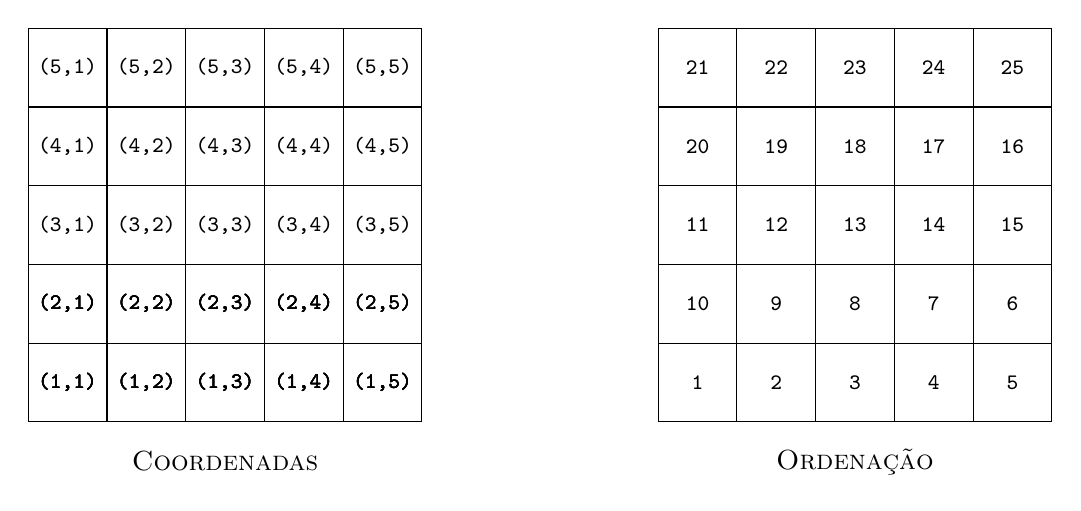
\begin{tikzpicture}

    \begin{scope}[shift={(0,0)}]
        \draw (0, 0) grid (5, 5);

        \node at (0.5, 0.5) { \footnotesize \tt (1,1) };
        \node at (1.5, 0.5) { \footnotesize \tt (1,2) };
        \node at (2.5, 0.5) { \footnotesize \tt (1,3) };
        \node at (3.5, 0.5) { \footnotesize \tt (1,4) };
        \node at (4.5, 0.5) { \footnotesize \tt (1,5) };

        \node at (0.5, 1.5) { \footnotesize \tt (2,1) };
        \node at (1.5, 1.5) { \footnotesize \tt (2,2) };
        \node at (2.5, 1.5) { \footnotesize \tt (2,3) };
        \node at (3.5, 1.5) { \footnotesize \tt (2,4) };
        \draw (0, 0) grid (5, 5);

        \node at (0.5, 0.5) { \footnotesize \tt (1,1) };
        \node at (1.5, 0.5) { \footnotesize \tt (1,2) };
        \node at (2.5, 0.5) { \footnotesize \tt (1,3) };
        \node at (3.5, 0.5) { \footnotesize \tt (1,4) };
        \node at (4.5, 0.5) { \footnotesize \tt (1,5) };

        \node at (0.5, 1.5) { \footnotesize \tt (2,1) };
        \node at (1.5, 1.5) { \footnotesize \tt (2,2) };
        \node at (2.5, 1.5) { \footnotesize \tt (2,3) };
        \node at (3.5, 1.5) { \footnotesize \tt (2,4) };
        \node at (4.5, 1.5) { \footnotesize \tt (2,5) };

        \draw (0, 0) grid (5, 5);

        \node at (0.5, 0.5) { \footnotesize \tt (1,1) };
        \node at (1.5, 0.5) { \footnotesize \tt (1,2) };
        \node at (2.5, 0.5) { \footnotesize \tt (1,3) };
        \node at (3.5, 0.5) { \footnotesize \tt (1,4) };
        \node at (4.5, 0.5) { \footnotesize \tt (1,5) };

        \node at (0.5, 1.5) { \footnotesize \tt (2,1) };
        \node at (1.5, 1.5) { \footnotesize \tt (2,2) };
        \node at (2.5, 1.5) { \footnotesize \tt (2,3) };
        \node at (3.5, 1.5) { \footnotesize \tt (2,4) };
        \node at (4.5, 1.5) { \footnotesize \tt (2,5) };

        \draw (0, 0) grid (5, 5);

        \node at (0.5, 0.5) { \footnotesize \tt (1,1) };
        \node at (1.5, 0.5) { \footnotesize \tt (1,2) };
        \node at (2.5, 0.5) { \footnotesize \tt (1,3) };
        \node at (3.5, 0.5) { \footnotesize \tt (1,4) };
        \node at (4.5, 0.5) { \footnotesize \tt (1,5) };

        \node at (0.5, 1.5) { \footnotesize \tt (2,1) };
        \node at (1.5, 1.5) { \footnotesize \tt (2,2) };
        \node at (2.5, 1.5) { \footnotesize \tt (2,3) };
        \node at (3.5, 1.5) { \footnotesize \tt (2,4) };
        \node at (4.5, 1.5) { \footnotesize \tt (2,5) };

        \node at (0.5, 2.5) { \footnotesize \tt (3,1) };
        \node at (1.5, 2.5) { \footnotesize \tt (3,2) };
        \node at (2.5, 2.5) { \footnotesize \tt (3,3) };
        \node at (3.5, 2.5) { \footnotesize \tt (3,4) };
        \node at (4.5, 2.5) { \footnotesize \tt (3,5) };

        \node at (0.5, 3.5) { \footnotesize \tt (4,1) };
        \node at (1.5, 3.5) { \footnotesize \tt (4,2) };
        \node at (2.5, 3.5) { \footnotesize \tt (4,3) };
        \node at (3.5, 3.5) { \footnotesize \tt (4,4) };
        \node at (4.5, 3.5) { \footnotesize \tt (4,5) };

        \node at (0.5, 4.5) { \footnotesize \tt (5,1) };
        \node at (1.5, 4.5) { \footnotesize \tt (5,2) };
        \node at (2.5, 4.5) { \footnotesize \tt (5,3) };
        \node at (3.5, 4.5) { \footnotesize \tt (5,4) };
        \node at (4.5, 4.5) { \footnotesize \tt (5,5) };

        \node at (2.5, -0.5) { \sc Coordenadas };
    \end{scope}

     \begin{scope}[shift={(8,0)}]
        \draw (0, 0) grid (5, 5);

        \node at (0.5, 0.5) { \footnotesize \bf \tt 1};
        \node at (1.5, 0.5) { \footnotesize \bf \tt 2};
        \node at (2.5, 0.5) { \footnotesize \bf \tt 3};
        \node at (3.5, 0.5) { \footnotesize \bf \tt 4};
        \node at (4.5, 0.5) { \footnotesize \bf \tt 5};

        \node at (0.5, 1.5) { \footnotesize \bf \tt 10};
        \node at (1.5, 1.5) { \footnotesize \bf \tt 9};
        \node at (2.5, 1.5) { \footnotesize \bf \tt 8};
        \node at (3.5, 1.5) { \footnotesize \bf \tt 7};
        \node at (4.5, 1.5) { \footnotesize \bf \tt 6};

        \node at (0.5, 2.5) { \footnotesize \bf \tt 11};
        \node at (1.5, 2.5) { \footnotesize \bf \tt 12};
        \node at (2.5, 2.5) { \footnotesize \bf \tt 13};
        \node at (3.5, 2.5) { \footnotesize \bf \tt 14};
        \node at (4.5, 2.5) { \footnotesize \bf \tt 15};

        \node at (0.5, 3.5) { \footnotesize \bf \tt 20};
        \node at (1.5, 3.5) { \footnotesize \bf \tt 19};
        \node at (2.5, 3.5) { \footnotesize \bf \tt 18};
        \node at (3.5, 3.5) { \footnotesize \bf \tt 17};
        \node at (4.5, 3.5) { \footnotesize \bf \tt 16};

        \node at (0.5, 4.5) { \footnotesize \bf \tt 21};
        \node at (1.5, 4.5) { \footnotesize \bf \tt 22};
        \node at (2.5, 4.5) { \footnotesize \bf \tt 23};
        \node at (3.5, 4.5) { \footnotesize \bf \tt 24};
        \node at (4.5, 4.5) { \footnotesize \bf \tt 25};

        \node at (2.5, -0.5) { \sc Ordenação };
    \end{scope}


    \end{tikzpicture}

\end{document}
